\section*{Question 3}
% Consider again the data used in Question 1. Let �Total Activities� be the
% response variable, and learn a decision tree for these data. Instances where �Total Activities� is higher
% than 40 should be mapped to class �High� and others should be mapped to class �Low�. The maximum
% depth of the tree should be set to three. After discovering the tree explain the result by explaining
% the resulting rules and interpreting the confusion matrix (this task should be done with RapidMiner).

The process
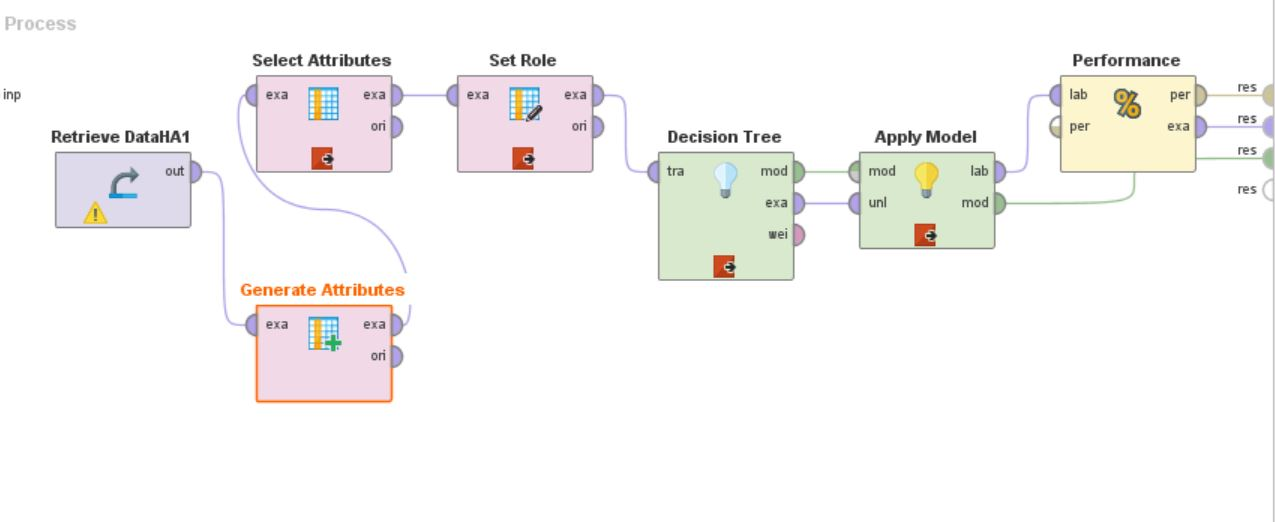
\includegraphics[width=\textwidth]{Question3Process.jpg}

first changes the numerical attribute TotalActivites to a nominal one by
\textbf{Generate Attributes} and \textbf{Select Attributes}. The generating
consideres the old TotalActivites and uses the rule that all data, where
TotalActivites is lower or the same as 40 it is assigned to ``Low'',
otherwise ``High''. The \textbf{Set Role} gives the new attribute role label,
so RapidMiner knows what should have to be the outcome of the Decision Tree.
\textbf{Decision Tree} generates the decision Tree. Then \textbf{Apply Model}
for \textbf{Performance} checking. The output is then the model and the
performance of the model on the data.

The resulting decision tree is 

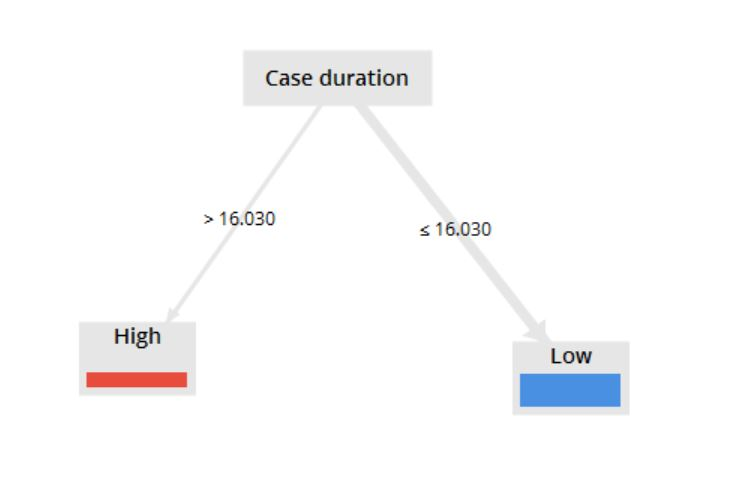
\includegraphics[width=\textwidth]{Question3Deci.jpg}

If you check the Confusionmatrix

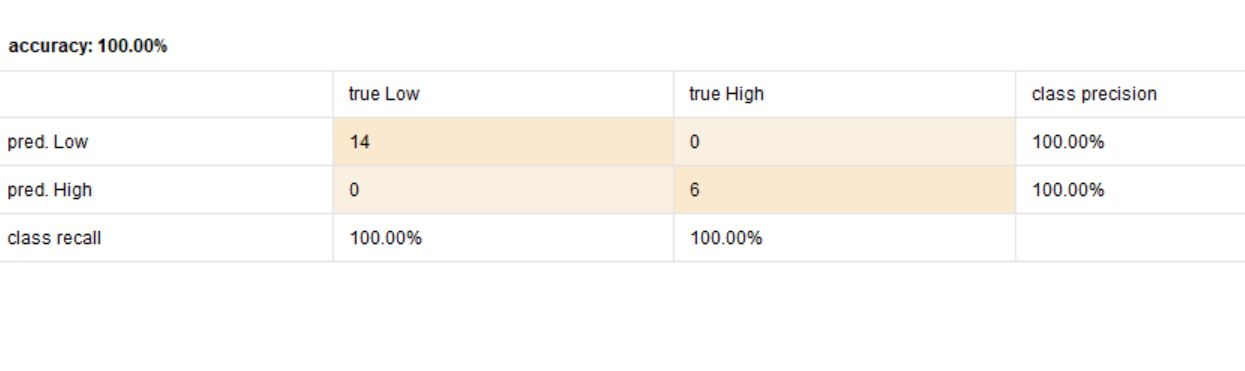
\includegraphics[width=\textwidth]{Question3Confusion.jpg}

you see, that this decision tree classifys the data perfectly. So you can
predict by just knowing the case duration the nominal outcome for total
activities.
If the case duration is higher, than also the total activities are high. This seems to be
logical, if you have to do a lot this takes most of the times longer and
otherwise around, if you do not need long you mostly did not do a lot of
different things in the time.


For completeness I checked also what happens for different setting:
\begin{enumerate}
  \item Changing case duration to nominal with high low (low, if
  caseduration<=1/6/15)\\
  \item Changing case duration to nominal with high,low,middel ((low, if
  caseduration<=6, middel if 6<caseduration<=15,otherwise high))
 \end{enumerate}
 The first case gives in all versions the same slightly different solution from
 the first one, but also it gets worse.
 
 The second version again gives a tree just deciding with the case duration.

 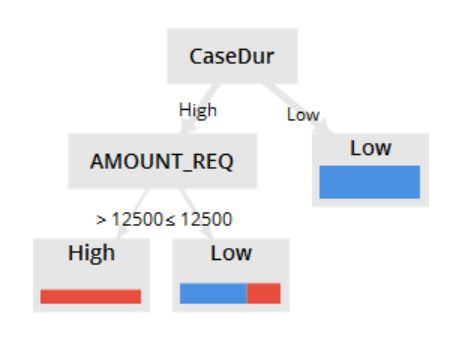
\includegraphics[width=\textwidth]{Question3DeciNew.jpg}
 
 I also treid what happens without case duration, but decided that this is not
 helpful for the exercise, because we have the information. In my opinion it is
 like said above a dependency bewtween duration and activity.
